\documentclass[11pt, twocolumn]{article}
\usepackage[a4paper,top=2.5cm,bottom=2.5cm,left=2cm,right=2cm,marginparwidth=1.75cm]{geometry}
\usepackage{graphicx}
\graphicspath{{3F1_figures/}}
\usepackage{mathptmx} % Times New Roman
\usepackage{caption}
\captionsetup{font=large, labelfont=bf, textfont=it, aboveskip=8pt, belowskip=2pt}

\begin{document}
\begin{figure}[h]
    \centering
    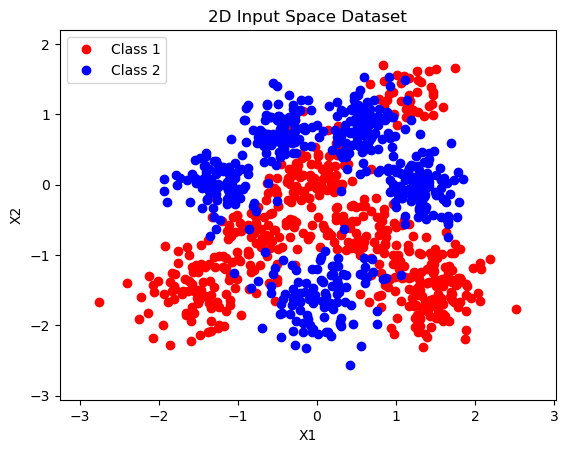
\includegraphics[width=\textwidth]{1}
    \caption{}
    \label{fig:1}
\end{figure}


\begin{figure}[h]
    \centering
    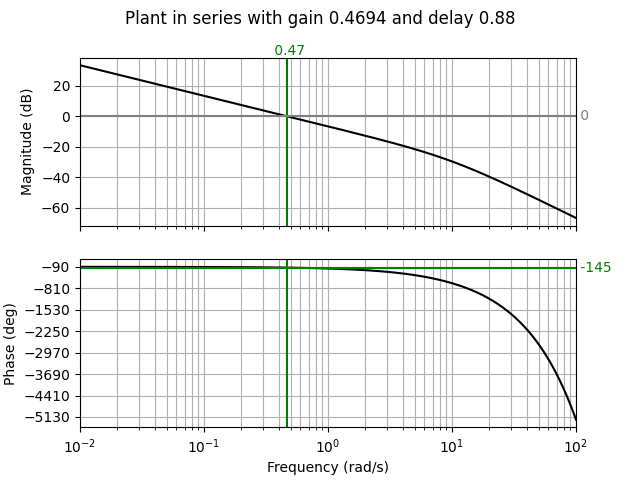
\includegraphics[width=\textwidth]{2}
    \caption{}
    \label{fig:2}
\end{figure}

\end{document}
